 We introduce several category theory notations foundational to the DPO graph transformation system discussed in this article.

\begin{definition}[Unlabelled graph \cite{barr1990category}] 
    An \textbf{unlabelled graph} \(G\) consists of a set of \textbf{nodes} (or \textbf{objects}) and a set of \textbf{arrows}, such that each arrow has a specific \textbf{source} (or \textbf{domain}) node and \textbf{target} (or \textbf{codomain}) node. A graph is \textbf{finite} if the number of nodes and arrows is finite.

    Given an unlabelled graph \(G\), we will systematically denote its vertices, arrows, source function, target function, domain function, and codomain function by \(G_0\), \(G_1\), \(\operatorname{source}\), \(\operatorname{target}\), \(\operatorname{dom}\), and \(\operatorname{cod}\), respectively. The notation \(a: s \mathop{\to} t\) signifies that \(a\) is an arrow from the source vertex \(s\) to the target vertex \(t\).
\end{definition}

\begin{definition}[Category \cite{barr1990category}]
    A (small) category is an unlabelled graph \(\mathcal{C}\) together with:
    \begin{itemize}
        \item a function \(u : \mathcal{C}_0 \mathop{\to} \mathcal{C}_1\),
        \item a partial function \(\star : \mathcal{C}_1 \mathop{\times} \mathcal{C}_1 \mathop{\to} \mathcal{C}_1\),
    \end{itemize}
    such that:
    \begin{itemize}
        \item for all arrows \(f:X \mathop{\rightarrow} Y\) and \(g:Y \mathop{\rightarrow} Z\), \(f \mathop{\star} g :X \mathop{\to} Z\) is defined;
        \item for every node \(X\), the source and target of \(u(X)\) are \(X\);
        \item for every \(f:X \mathop{\rightarrow} Y\), we have \(u(X) \mathop{\star} f \mathop{=} f \mathop{=} f \mathop{\star} u(Y)\);
        \item for all arrows \(f, g\), and \(h\), we have \((f \mathop{\star} g) \mathop{\star} h \mathop{=} f \mathop{\star} (g \mathop{\star} h)\) whenever either side is defined.
    \end{itemize}
 
    Arrows are called \textbf{morphisms}. The function $\star$ is called \textbf{composition}. If $X$ is an object of $\mathcal{C}$, the arrow $u(X)$ is denoted $\operatorname{id}_X$, which is called the \textbf{identity} of the object $X$. 
\end{definition}

\begin{remark}
    The composite of morphisms \( f: X \mathop{\to} Y \) and \( g: Y \mathop{\to} Z \) is denoted by \( f \mathop{\star} g \) instead of \( g \circ f \) as commonly found in the literature.
\end{remark}

\input{\nonWFonly/sections/preliminaries_category_theory_mono_relativeMono}

\begin{definition}[Span \cite{lowe2010graph} and Cospan ]
    An ordered pair \(( \alpha : A \mathop{\to} B, \beta : A \mathop{\to} C )\) of morphisms with the same domain is called a \textbf{span}, denoted as \( B \overset{\alpha}{\leftarrow} A \overset{\beta}{\rightarrow} C \). 
    An ordered pair \(( \beta' : B \mathop{\to} D, \alpha' : C \mathop{\to} D )\) of morphisms with the same codomain is called a \textbf{cospan}, denoted as \( B \overset{\beta'}{\rightarrow} D \overset{\alpha'}{\leftarrow} C \). 
\end{definition}

\begin{definition}[Diagram \cite{barr1990category}]
    Let \(G\) be a graph and \(\mathcal{C}\) a category. A \textbf{diagram} in \(\mathcal{C}\) of shape \(G\) is a homomorphism \(h : G \mathop{\to} \mathcal{C}\). A diagram is said to be \textbf{commutative} if for any nodes \(u\) and \(v\) and any two paths from \(u\) to \(v\)

    \begin{center}
    \resizebox{12cm}{!}{
        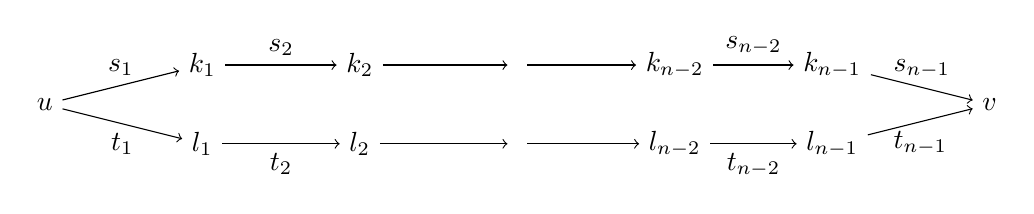
\begin{tikzpicture}
        \node (u) at (0,0) {\(u\)};
        \node (k1) at (2,0.5) {\(k_1\)};
        \node (k2) at (4,0.5) {\(k_2\)};
        \node (ketc) at (6,0.5) {\(\hdots\)};
        \node (knm2) at (8,0.5) {\(k_{n-2}\)};
        \node (knm1) at (10,0.5) {\(k_{n-1}\)};
        \node (v) at (12,0) {\(v\)};
        \node (l1) at (2,-0.5) {\(l_1\)};
        \node (l2) at (4,-0.5) {\(l_2\)};
        \node (letc) at (6,-0.5) {\(\hdots\)};
        \node (lnm2) at (8,-0.5) {\(l_{n-2}\)};
        \node (lnm1) at (10,-0.5) {\(l_{n-1}\)};
        \draw[->] (u) -- (k1) node [midway,above] {\(s_1\)};
        \draw[->] (k1) -- (k2) node [midway,above] {\(s_2\)};
        \draw[->] (k2) -- (ketc);
        \draw[->] (ketc) -- (knm2); 
        \draw[->] (knm2) -- (knm1) node[midway,above] {\(s_{n-2}\)}; 
        \draw[->] (knm1) -- (v) node[midway,above] {\(s_{n-1}\)}; 
        \draw[->] (u) -- (l1) node[midway,below] {\(t_1\)};
        \draw[->] (l1) -- (l2) node[midway,below] {\(t_2\)};
        \draw[->] (l2) -- (letc);
        \draw[->] (letc) -- (lnm2); 
        \draw[->] (lnm2) -- (lnm1) node[midway,below] {\(t_{n-2}\)}; 
        \draw[->] (lnm1) -- (v) node[midway,below] {\(t_{n-1}\)}; 
        \end{tikzpicture}
    }
    \end{center}
    \noindent
    it holds that \(h(s_1) \mathop{\star} h(s_2) \mathop{\star} \hdots \mathop{\star} h(s_{n-2}) \mathop{\star} h(s_{n-1}) \mathop{=} h(t_1) \mathop{\star} h(t_2) \mathop{\star} \hdots \mathop{\star} h(t_{n-2}) \mathop{\star} h(t_{n-1})\).
\end{definition}
\begin{definition}[Pushout \cite{barr1990category} \cite{overbeek2023graph}]
    \begin{figure}[htbp] 
        \center
        \begin{subfigure}[b]{0.38 \textwidth}
            \center
            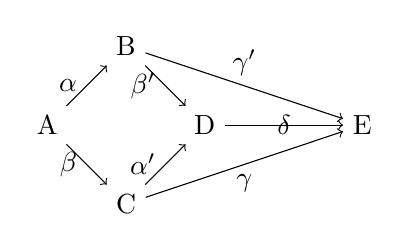
\begin{tikzpicture}
                \node (i) at (0,0) {A};
                \node (r) at (1,1) {B};
                \node (c) at (1,-1) {C};
                \node (h) at (2,0) {D};
                % \node () at (1,-1) {\( \Delta \)};
                \draw[->]  (i) -- (r) node [midway,left] {$\alpha$};
                \draw[->] (c) -- (h) node [midway,left] {$\alpha'$};
                \draw[->] (r) -- (h) node[midway, left] {$\beta'$};
                \draw[->] (i) -- (c) node[midway, left] {$\beta$};
                \node (d') at (4,0) {E};
                \draw[->] (c) -- (d') node [midway,below]{$\gamma$};
                \draw[->] (r) -- (d') node [midway,above]{$\gamma'$};
                \draw[->] (h) -- (d') node [midway]{$\delta$};
            \end{tikzpicture}
            \caption{pushout}
            \label{diag:def_pbpo_po}
        \end{subfigure}
        \caption{}
        \label{fig:def_pb_po}
    \end{figure}
    A \textbf{pushout} of a span \( B \overset{\alpha}{\leftarrow} A \overset{\beta}{\rightarrow} C \) is defined as a cospan \( B \overset{\beta'}{\rightarrow} D \overset{\alpha'}{\leftarrow} C \) such that for every cospan \( B \overset{\gamma'}{\rightarrow} E \overset{\gamma}{\leftarrow} C \) satisfying \(\alpha \mathop{\star} \gamma' \mathop{=} \beta \mathop{\star} \gamma\), there exists a unique morphism \(\delta\) that makes the commutative diagram in~\autoref{diag:def_pbpo_po} valid. The diagram involving \(\alpha\), \(\beta\), \(\alpha'\), and \(\beta'\) is referred to as the \textbf{pushout square}, \(D\) as the \textbf{pushout object}, and the existence of the unique morphism is known as the \textbf{universal mapping property of the pushout}.
\end{definition}

Sets with functions between sets constitute the category \(\mathbf{Set}\). Pushouts always exist in \textbf{Set}, and are unique up to isomorphism.

\begin{example}
    Given a span \( B \overset{\alpha}{\leftarrow} A \overset{\beta}{\rightarrow} C \) in \textbf{Set}, a pushout can be constructed as follows:
    Define the pushout set as
    \(
     (B \biguplus C) / \sim
    \)
    where \(\sim\) is the equivalence relation on \(B \mathop{\times} C\) defined such that \( b \sim c \) if and only if there exists an \(a \mathop{\in} A\) for which \(\alpha(a) \mathop{=} b\) and \(\beta(a) \mathop{=} c\). Then, define the cospan as \( (\beta',\alpha') \), where \(\beta'\) and \(\alpha'\) map elements to their corresponding equivalence classes.
\end{example}